\documentclass{article}

% Encodings, page setup, paragraph formatting, font
\usepackage[top=0.9in, bottom=1in, left=1.5in, right=1.5in]{geometry}
\usepackage[utf8]{inputenc}
\usepackage[icelandic]{babel}
\usepackage[T1]{fontenc}
\usepackage{mathpazo}
\usepackage[parfill]{parskip}
% Tables and lists
\usepackage{booktabs,tabularx}
\usepackage{multirow, multicol}
\usepackage{enumerate}
% Math
\usepackage{amsmath, amsfonts, amssymb, amsthm}
% Graphics
\usepackage{graphicx}
\usepackage{tikz}
% Code environment
\usepackage{minted}
% Hyperlinks and related
\usepackage[pdftex,bookmarks=true,colorlinks=true,pdfauthor={Eirikur Ernir Thorsteinsson},linkcolor=blue,urlcolor=blue]{hyperref}

% Minted configuration
\usemintedstyle{default}
\renewcommand{\theFancyVerbLine}{\sffamily \arabic{FancyVerbLine}}

\floatstyle{plaintop}
\newfloat{program}{thp}{lop}
\floatname{program}{Forrit}
% End minted configuration

% Picture locations
\graphicspath{{./Pics/}}

% Meta information
\date{}
\author{Eiríkur Ernir Þorsteinsson}
\newcommand{\semester}{vor 2017}
\newcommand{\Semester}{Vor 2017}

% Hyphenation
\hyphenpenalty=5000
% Page and section numbering
\setcounter{secnumdepth}{-1} 
\pagenumbering{gobble}

\title{Tölvunarfræði 2, \semester \\ Námsáætlun og upplýsingar}
\author{}

\begin{document}
\maketitle
\hypersetup{pdftitle={Tölvunarfræði 2 - \semester}}

\section{Námsáætlun}
\label{sec:schedule}

Námskeiðið er framhaldsnámskeið Tölvunarfræði 1. Í upphafi námskeiðins er farið dýpra í hlutbundna forritun í Java-forritunarmálinu. Nemendur sem lærðu önnur forritunarmál en Java í sínu fyrsta forritunarnámskeiði eru hvattir til að kynna sér grundvallaratriði Java við fyrsta tækifæri. Aðalviðfangsefni námskeiðsins, gagnagrindur og reiknirit sem á þeim vinna, koma fyrir í framhaldinu. Sjá  töflu \ref{tab:schedule}.

\begin{table}
\caption{Námsáætlun eftir vikum}
\label{tab:schedule}
\begin{center}
\renewcommand{\arraystretch}{1.2}
\begin{tabularx}{\linewidth}{lcXp{1cm}}
\toprule
Vika&Dagsetning&Námsefni&Kafli\\
\midrule
1	&13/1	& Kynning á námskeiðinu, upprifjun á Java, minnismeðhöndlun, notkun safna, villumeðhöndlun&\\
2	&20/1	& Hlutbundin forritun í Java, erfðir&\\
3	&21/1	& Fjölnota klasar?&\\
4	&27/9	& ?&\\
5	&3/2	& Skjóður, biðraðir, hlaðar, greining reiknirita&Alg 1\\
6	&10/2	& Röðunarreiknirit&Alg 2\\
7	&17/2	& Röðunarreiknirit, forgangsbiðraðir&Alg 2\\
8	&24/2	& Leit, leitartré&Alg 3\\
9	&3/3	& Leitartré, hakkatöflur&Alg 3\\
10	&10/3	& Net, stefnd net&Alg 4\\
11	&17/3	& Minnstu spanntré, stystu vegir&Alg 4\\
12	&24/3	& Strengir, trie&Alg 5\\
13	&31/3	& Strengjaleit, reglulegar segðir&Alg 5\\
14	&7/4	& Skekkjumörk í námsáætlun&-\\
15	&14/4	& Páskaleyfi&-\\
16	&21/4	& ?&-\\
\bottomrule
\end{tabularx}
\end{center}
\end{table}

\section{Kennari}
Aðalkennari er Eiríkur Ernir Þorsteinsson. Aðsetur er í Tæknigarði, 2. hæð, stofa 212. Sjá mynd \ref{fig:taeknigardur}.

Til að hafa samband við kennara er ráðlagt að setja inn þráð á \href{???}{Piazza}. Allar fyrirspurnir sem ekki fela í sér persónulegar upplýsingar ættu að fara þangað. 

Tölvupóstfang er \href{mailto:ernir@hi.is}{ernir@hi.is}.

\begin{figure}
\caption{Önnur hæð í Tæknigarði. Kennara má finna í stofu 212.}
\label{fig:taeknigardur}
\begin{center}
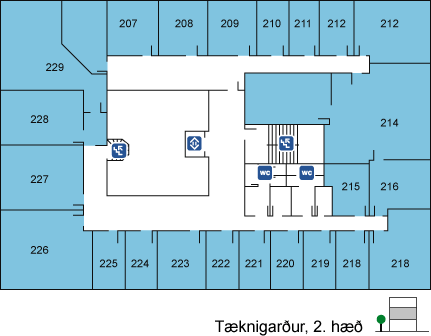
\includegraphics[width=0.5\linewidth]{taeknigardur}
\end{center}
\end{figure}

\section{Tímar og námstilhögun}
Aðalkennsla fer fram í vikulegum fyrirlestri. Fyrirlestrarnir eru %á föstudögum frá 10:00 til 12:20 í Háskólabíói, sal 1.

%Dæmatímar eru á mánudögum og þriðjudögum, ætlaðir til stuðnings fyrir skilaverkefni. Dæmahópum er úthlutað eftir fögum og stundatöflum, nemendur eru vinsamlegast beðnir um að mæta í úthlutaðan dæmatíma ef kostur er til að dreifingin á milli hópa sé sem jöfnust.

\subsection{Mætingaskylda}
Ekki er skylda að mæta í fyrirlestra eða dæmatíma (en sjá \nameref{sec:lecture-exercises}). Nemendur eru ábyrgir fyrir því að forgangsraða tíma sínum.
\subsection{Upptökur á fyrirlestrum}
Fyrirlestrar eru teknir upp þegar tæknin leyfir. Varað er við því að treysta á upptökur í stað mætingar í fyrirlestra.

\section{Námsbækur}
Aðalkennslubók er \emph{Algorithms}, fjórða útgáfa, eftir Sedgewick og Wayne. %Kennsla eftir þeirri bók hefst í fjórðu kennsluviku, eftir kynningu á C++ (sjá \nameref{tab:schedule}). 

%Til stuðnings við er bent á \emph{C++ in One Hour a Day}, 8. útgáfa, eftir Siddhartha Rao. Litið verður til hennar við yfirferð á C++, en ekki verður vísað beint í bókina.

\begin{figure}
\caption{Kennslubók}
\begin{center}
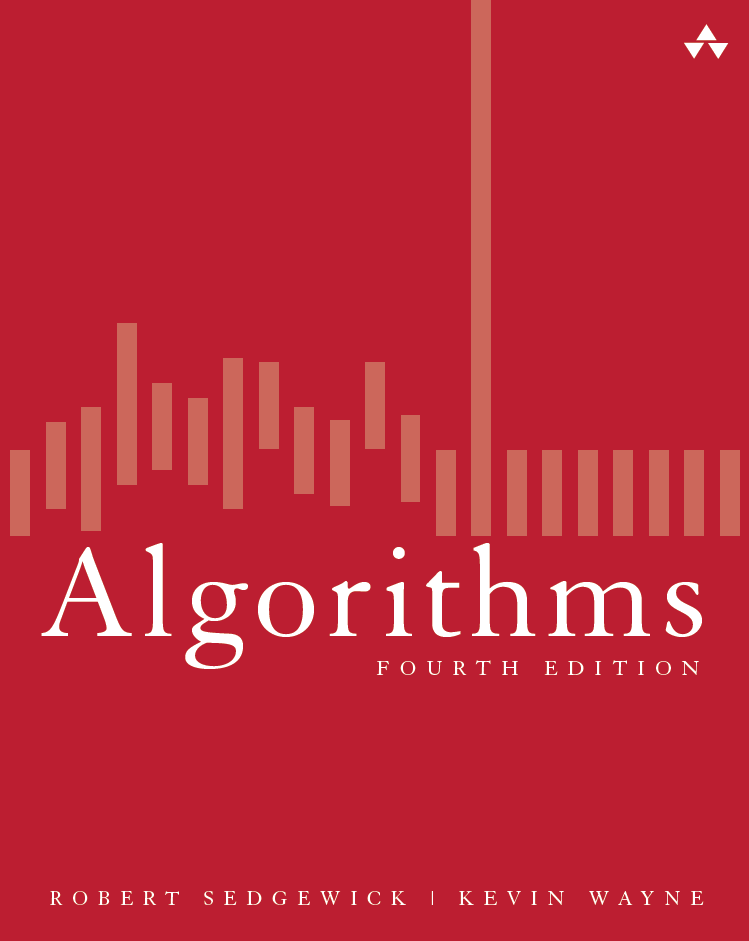
\includegraphics[height=8cm]{algorithms4th}
\end{center}
\end{figure}

\newpage
\section{Námsmat, einkunnir og próf}
\subsection{Fyrirlestraræfingar}
\label{sec:lecture-exercises}
Fyrirlestraræfingar eru í hverjum föstudagsfyrirlestri. Vægi þeirra er 10\% af lokaeinkunn. Þátttaka í $n$ fyrirlestraræfingum gefur hluteinkunnina $n$, að hámarki 10.

Tenglar á fyrirlestraræfingar verða gerðir aðgengilegir í hverri viku. Fyrirlestraræfingarnar verða nafni sínu samkvæmt hannaðar til að vera leystar í fyrirlestrartímunum sjálfum, en miðað verður við að hver þeirra verði opin í um það bil sólarhring.
\subsection{Skilaverkefni}
Vikuleg verkefnaskil eru í námskeiðinu. Meðaleinkunn 10 bestu skilaverkefnanna er 20\% af lokaeinkunn. Verkefnunum skal skila á Gradescope.com (sjá \nameref{sec:tools}). Ekki er tekið við seinum skilum.

Nauðsynlegt er að skila fjórum af fyrstu sex skilaverkefnunum til að öðlast próftökurétt.
\subsection{Próf}
Vægi lokaprófs er 70\% af lokaeinkunn. Leyfilegt verður að taka með eitt blað af glósum (skrifað á báðar hliðar) í lokapróf.

Lágmarkseinkunn er 5. Nauðsynlegt er að ná lágmarkseinkunn á lokaprófi sem og í námskeiðinu sem heild til að standast námskeiðið. 

Ekki er miðmisserispróf í námskeiðinu.
\section{Kennslutól}
\label{sec:tools}
Vefkennslutól verða notað eftir föngum. Mælt er með að nemendur skrái sig inn á eftirfarandi þjónustur sem allra fyrst:
\begin{itemize}
 \item \href{https://piazza.com/hi.is/spring2017/tl203g/home}{Piazza} er fyrirspurnavefurinn sem notaður er í námskeiðinu. Skráningin í námskeiðið á að vera sjálfvirk, en hafi það misfarist á að vera hægt að skrá sig handvirkt. Allar spurningar sem snúa að námskeiðinu ættu að fara inn á Piazza frekar en í tölvupóst.
 \item \href{https://gradescope.com/courses/5640}{Gradescope.com} er vefkerfið sem notað er til að taka við skilaverkefnum. Nemendur þurfa að skrá sig sjálfir á þennan vef. Aðgangskóði námskeiðsins er \texttt{95434M}. Mikilvægt er að skrá sig á Gradescope með fullu nafni (íslenskir stafir eru leyfilegir) og með því að nota HÍ-netfang. Kerfið tekur við \texttt{.pdf} skrám.
\end{itemize}
Fyrir utan vefkennslutól er nauðsynlegt að nemendur setji upp þýðanda fyrir Java ásamt viðeigandi ritli á eigin tölvu eða útvegi sér aðgang að slíkri vél.

\section{Undanþágur og sérúrræði}

\vfill

\includegraphics[width=0.5\linewidth]{hi-von-logo}
\end{document}